\chapter{Segunda Iteración}

Como se explica en el la subsección \ref{metodologiadedesarrollo}, en la que se expone la metodología de desarrollo utilizada para el proyecto, este sufre de tres grandes iteraciones para su completitud. En esta sección se explican los detalles implementados en la segunda iteración, es decir, la generación de un mejor diseño de la aplicación, nuevas interfaces, refactorización de clases y código replicado, así como mejoras gráficas visuales dentro de la aplicación, incluyendo referencias a la sección \ref{primeraiteracion}, explicando los cambios en diseño y comportamiento.

\section{Arquitectura del Proyecto}
\label{it2arquitectura}

La arquitectura del proyecto ha cambiado radicalmente desde la primera iteración, en la que estaba centrada en cómo se debería tratar el documento de especificación de juego, incluido dentro del paquete del juego, en forma de XML para que, cada elemento fuese lo más dinámico posible y sostenible. A su vez, estaba centrada en la clase Game, y existían multitud de clases, llamadas clases de utilidad, que contenían funcionalidad que debía ser accesible a través de una clase controladora de nivel superior.

En esta arquitectura encontramos tres paquetes importantes que engloban la funcionalidad necesaria para la ejecución del proyecto. Están representados en la figura \ref{arquitecturait2} Estos tres paquetes son:

\begin{itemize}
	\item \textbf{Core}: \textit{Core} contiene el núcleo de eAdventure portado a Unity. Este paquete está formado, a su vez, por varios subpaquetes. El primero de ellos es \textit{DataModel}, donde se encuentra todo el modelo de datos portado de eAdventure a Unity, siendo completamente fiel a la implementación realizada en Java, y soportando todas las funcionalidades que se soportaban en dicho editor. El segundo de ellos es \textit{Loader}, donde está contenido el nucleo de lectura y carga del fichero XML de especificación del juego. Este \textit{Loader}, recibe un XML y genera un objeto \textit{AdventureData} que contiene todos los datos del juego. Por último, dentro de \textit{Core} encontramos un paquete \textit{Auxiliar} con clases útiles para este modelo de datos.
	
	\item \textbf{RAGETracker}: que contiene los elementos necesarios para generar un registro de actividad de juego del usuario y comunicarse con RAGE a través de Unity. RAGE se encarga de realizar tareas de evaluación y \textit{Learning Analytics} mediante el análisis de las trazas producidas por el alumno mientras juega. Esto permite al profesor que esté utilizando un juego producido con uAdventure, que se beneficie de las ventajas de RAGE, pudiendo reforzar aquellos alumnos que estén teniendo un desarrollo insuficiente o anormal en el juego.
	
	\item \textbf{Runner}: que se encarga de la transformación desde la especificación una ruta donde hay un juego descomprimido, hasta la generación de un entorno gráfico interactivo que permite al usuario jugar al juego. Contiene 3 subpaquetes que se encargan de diferentes tareas. En primer lugar, el paquete ResourceManager, que se encarga de la carga transparente de recursos, ya sean imágenes, videos, botones, cursores, u otros elementos multimedia. En segundo lugar, el paquete Appearance, que se encarga de mejorar la visualización, mediante diferentes formas de mostrar burbujas de diálogo, o mediante el uso de Shaders. Por último, el paquete \textit{GameLogic and Representation} que se encarga de ejecutar la lógica del juego. Este contiene en su interior una serie de gestores y controladores que son capaces de controlar la ejecución del juego, junto a las secuencias, trayectorias, así como una serie de comportamientos que tomarán lugar dentro de la escena.
\end{itemize}

\begin{figure}[h!]
	\centerline{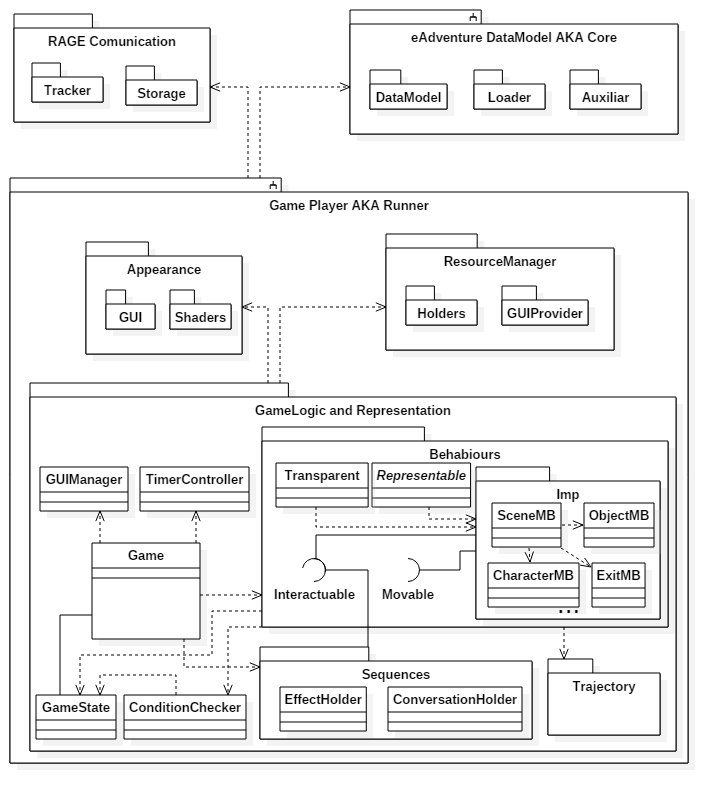
\includegraphics[height=7.5in]{figures/it2/Arquitectura.png}}
	\caption[Arquitectura - Versión Final]{Arquitectura del sistema, a nivel de paquetes de la versión final del proyecto}
	\label{arquitecturait2}
\end{figure}

\newpage

\section{El nucleo de Ejecución: Runner}

El núcleo de ejecución, también conocido como \textit{Runner}, está dividido en 3 subpaquetes, \textit{Apearance}, encargado de mejorar la representación visual, \textit{ResourceManager}, encargado de realizar la carga transparente de recursos, y \textit{GameLogic}, el cual podría considerarse el núcleo en si mismo, de lógica del juego. Estos tres paquetes surgen de la generalización de elementos que se encontraban, o bien en la antigua clase \textit{Game}, explicada en la sección \ref{gameit1}, o bien en alguna de las clases de utilidad, explicadas en la sección \ref{utilit1}.

De esta manera conseguimos que, la antigua clase controladora del juego \textit{Game}, y las Clases de Utilidad, ahora no tenga que realizar tantas tareas como realizaba anteriormente. En su lugar surgen 5 clases. Estas clases se encargan de hacer transparente la gestión de diversas tareas. Algunas de ellas realizan la gestión de un elemento en concreto, otras controlan la ejecución de otros elementos, y, por último otras se encargan de gestionar el estado del juego.

Estas 5 clases son:
\begin{enumerate}
	\item \textbf{Game}: La clase Game ha sido reducida para encargarse de tres tareas principales: En primer lugar, iniciar la carga y poner en funcionamiento el juego una vez esté cargado. En segundo lugar, controlar la interacción del usuario con los elementos del juego, ya sean elementos con representación, o elementos abstractos como secuencias. Y por último, ser la puerta de enlace que permite elegir qué escena se va a representar.
	
	\item \textbf{GUIManager}: Este gestor se encarga de realizar la gestión de la interfaz que antes se realizaba en \textit{Game}. Permite la emisión de burbujas de diálogo y el control sobre ellas, la posibilidad de mostrar una lista de opciones entre las que el usuario debe seleccionar una respuesta, y por último, la representación de acciones, como botones, y la gestión del menú contextual.
	
	\item \textbf{GameState}: Aunque \textit{GameState} no se considere un \textit{Manager} en si mismo, porque, a diferencia de todos los demás, no es un Singleton, siempre sigue habiendo una única Instancia, pues solo podemos tener un estado de juego, excepto cuando cargamos y guardamos partida. Maneja el estado del juego, que antes se realizaba en \textit{Game}, y facilita funciones para acceder a objetos de la especificación del juego, como \textit{Item} o \textit{NPC}.
	
	\item \textbf{TimerController}: Este gestor que se encarga de controlar los temporizadores que se utilizan en uAdventure para determinadas tareas, como, por ejemplo, hacer que un edificio se queme si no se ha evacuado a tiempo, es, tanto un \textit{Singleton}, como un \textit{MonoBehaviour}, pues necesita de la función \textit{Update()} para controlar que sus temporizadores no hayan saltado. Esta funcionalidad no estaba disponible en la anterior iteración.
	
	\item \textbf{ResourceManager}: este gestor se encarga de facilitar un repositorio transparente a través del cual acceder a los recursos del juego. Añade funcionalidades adicionales que no estaban disponibles anteriormente, como la persistencia en memoria de recursos para agilizar los tiempos de carga, la carga de vídeos, así como la carga de archivos de sonido.
\end{enumerate}

La representación de las clases que se explican en esta sección está disponible en la figura \ref{runnerbigit2}, junto a todas sus funciones. En este diagrama no están representados todos los elementos, pero si aquellos que han surgido de la evolución de las clases que se especificaron al comienzo de la sección. Este diagrama es bastante específico, pues contiene datos acerca de todas las funciones disponibles en cada uno de los elementos.

\newpage

\begin{figure}[h!]
	\centerline{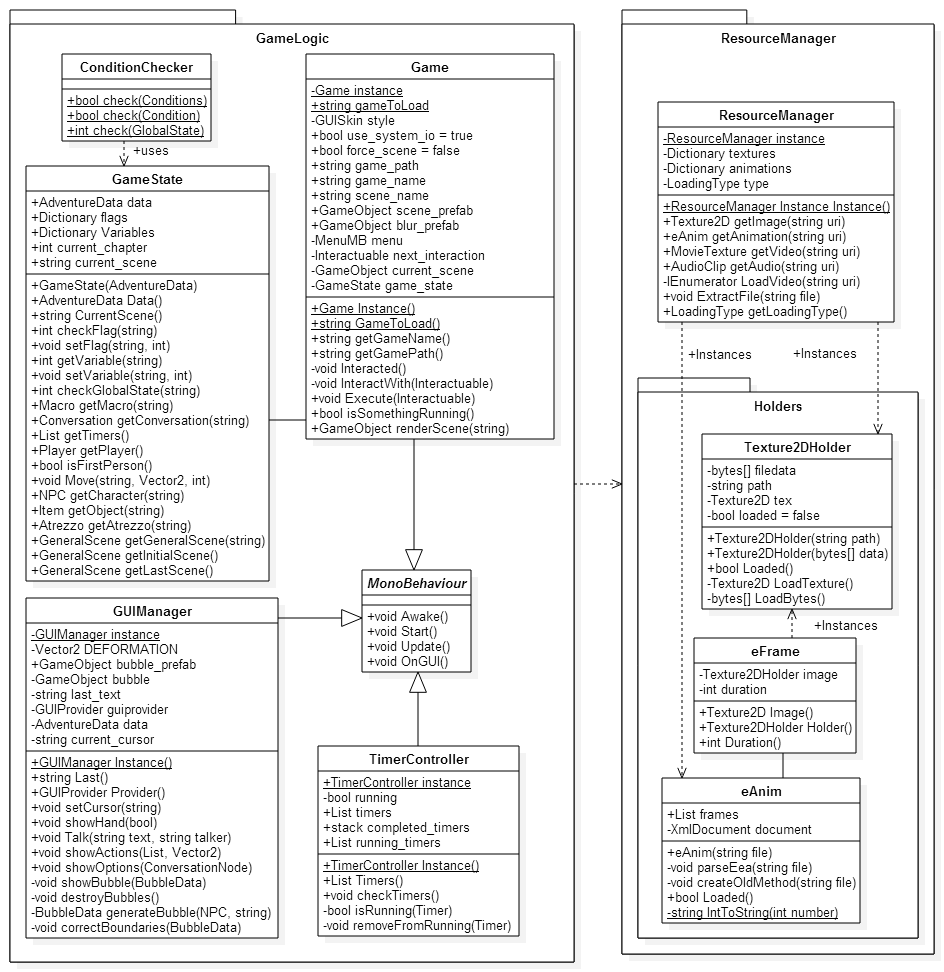
\includegraphics[height=7.5in]{figures/it2/GameLogicBigOnes.png}}
	\caption[GameLogic Grandes Gestores - Versión Final]{Diagrama de clases de los grandes gestores que controlan y proveen contenido para la ejecución del juego.}
	\label{runnerbigit2}
\end{figure}

\newpage

\subsection{El gestor de interfaz: GUIManager}

Como se explica en la sección superior a esta subsección, existe una clase gestora que se encarga de manejar la interfaz en su totalidad de forma transparente. Facilita una serie de funciones que permiten, de forma sencilla, mostrar burbujas de diálogo, cambiar el cursor, mostrar un menú contextual de acciones, o un menú de opciones.

Este gestor surge de la reducción de contenido de \textit{Game}, que antes realizaba estas tareas, y fue relevada de su función debido a que dicha clase comenzaba a tener una dimensión demasiado elevada. La figura \ref{guimanagerit2} muestra el diagrama de clases de la clase \textit{GUIManager} junto al paquete \textit{Apearance}, el paquete \textit{GUIProvider} que contiene todo lo necesario para acceder al \textit{ResourceManager} de forma automática y transparente, así como la carga de recursos por defecto y la gestión de nombres a constantes y viceversa, y el paquete \textit{Menu}, que contiene una serie de clases para la representación y animación del Menú.

Este gestor hereda de \textit{MonoBehaviour}, por lo que es asignado como componente de un elemento dentro de la escena. En este caso se asigna a un objeto \textit{Canvas}, que permite la representación de elementos de interfaz. 

El ciclo de vida de \textit{GUIManager} comienza cuando despierta la escena. En este momento se establece como instancia a si mismo. Tras esto, cuando \textit{Game} ya ha cargado el juego, y se ejecuta la función \textit{Start()}, este provee al \textit{GUIProvider} de los datos del juego en forma de un \textit{AdventureData}. Este se prepara y carga los recursos que deba cargar, y tras esto, el \textit{GUIManager} se queda en espera hasta que el juego necesite mostrar al usuario algo.

Una vez que el \textit{GUIManager} se encuentra en espera, facilita una serie de funciones útiles para representar cosas al usuario, estas son:
\begin{itemize}
	\item \textbf{Talk(string line, string talker)}: Esta función permite al sistema que los personajes hablen. Esto se ha implementado mediante el uso de burbujas.
	
	\item \textbf{showActions(List<Actions>, Vector2 position)}: Esta función pone en ejecución al menú contextual, y hace que se muestre con las acciones especificadas en una posición.
	
	\item \textbf{showOptions(ConversationNode)}: Esta función permite mostrar un listado de opciones de texto que el usuario debe elegir. Adicionalmente, el fondo se emborrona y se muestra el texto de la última pregunta.
	
\end{itemize}


\begin{figure}[h!]
	\centerline{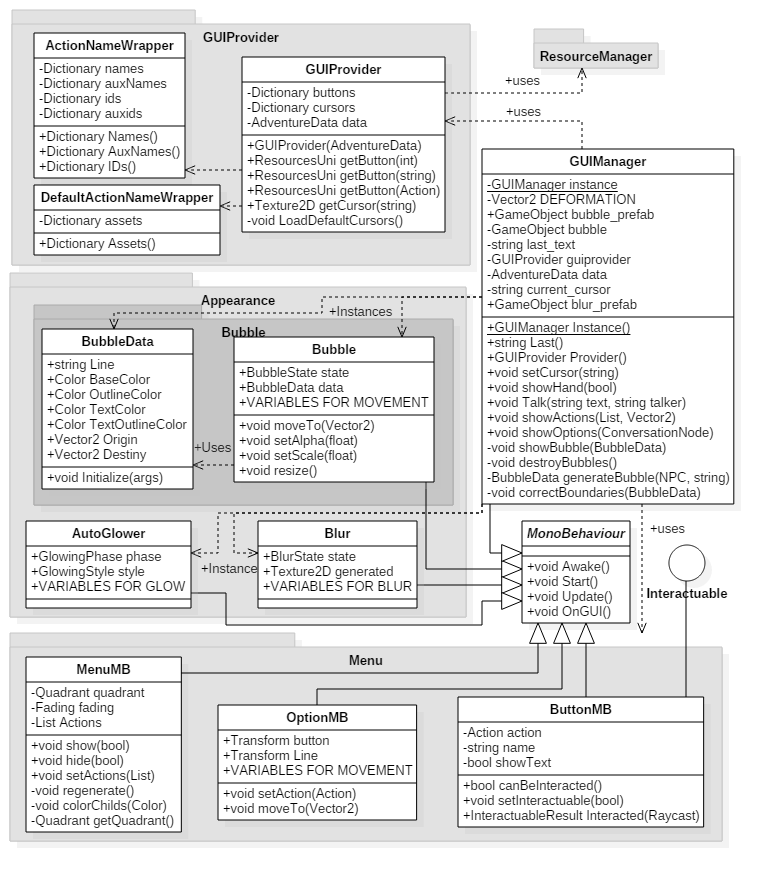
\includegraphics[height=7.5in]{figures/it2/GUIManager.png}}
	\caption[GameLogic Grandes Gestores - Versión Final]{Diagrama de clases de los grandes gestores que controlan y proveen contenido para la ejecución del juego.}
	\label{guimanagerit2}
\end{figure}

\newpage

\subsubsection{Proveedor de recursos de GUI: GUIProvider}

La interfaz es una capa de la vista que necesita representación, y por ello, necesita acceder a recursos para poder representarse. Sin embargo, nuestro gestor de \textit{GUI} no usa directamente al \textit{ResourceManager}, sino que utiliza una clase intermedia para acceder a los recursos, esta clase es \textit{GUIProvider}, y se encarga de, facilitar el acceso a texturas que tengan una funcionalidad concreta. Es decir, por ejemplo, obtener la textura que representa a una acción, o el cursor que se debe mostrar para un determinado elemento. \textit{GUIProvider} se encarga de proveer los recursos apropiados.

Además de esto, eAdventure sigue una jerarquía a la hora de definir recursos para la interfaz, esta es la siguiente:

\begin{enumerate}
	\item Se cargan los recursos por defecto. Estos recursos están repartidos en dos directorios, el primero es la carpeta "~/gui/hud/contextual/" donde se encuentran los botones que representan los distintos tipos de acciones y que se obtienen utilizando la clase \textit{DefaultActionNameWrapper}. El segundo el la carpeta "~/gui/cursors/" donde se encuentran los cursores del juego, y que se obtienen utilizando la clase \textit{ActionNameWrapper}. Estas dos clases \textit{Wrapper} se encargan de transformar de Acción, o identificador de Acción a nombre, y viceversa.
	
	\item Se cargan los recursos especificados en la base del archivo "descriptor.xml". Tras la lectura de dicho archivo en \textit{Loader}, estos se encuentran en el objeto de datos \textit{AdventureData} que gestiona \textit{GameState}. Estos también se asignan utilizando los \textit{Wrappers} anteriormente especificados, y, sustituyen a los botones y cursores cargados en el apartado anterior con los que se hayan en esta especificación.
	
	\item Por último puede ocurrir una situación anómala, y es que un elemento tenga una acción personalizada en su interior. En este caso, y excepcionalmente, es el propio botón del menú el que se encarga de solicitar al \textit{ResourceManager} dichos recursos.
	
\end{enumerate}

\begin{figure}[h!]
	\centerline{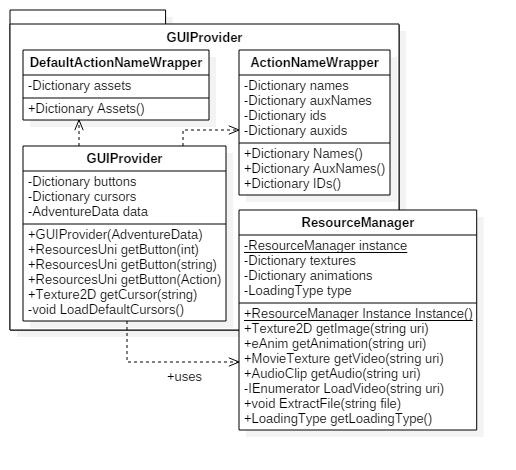
\includegraphics[height=3.5in]{figures/it2/GUIProvider.png}}
	\caption[GUIProvider - Versión Final]{Diagrama de clases de GUIProvider, junto con ResourceManager.}
	\label{guiproviderit2}
\end{figure}

Las clases que participan en este proceso están representadas en la figura \ref{guiproviderit2}. En esta figura, aunque \textit{ResourceManager} esté sobrepuesto al paquete \textit{GUIProvider}, esto es debido a reducir el tamaño del diagrama, realmente este no forma parte de dicho paquete.

\subsubsection{Las burbujas de diálogo: Bubble}

La representación de diálogos en un juego de aventuras es una tarea necesaria, pues los personajes necesitan hablar para compartir información entre ellos. La manera de representar estos diálogos en uAdventure es la misma que se decidió utilizar en eAdventure: Las burbujas de diálogo, o bocadillos de diálogo. Sin embargo, estas burbujas han evolucionado en su representación, realizando una pequeña animación a la hora de ser invocadas, y a la hora de desaparecer.

\begin{figure}[h!]
	\centerline{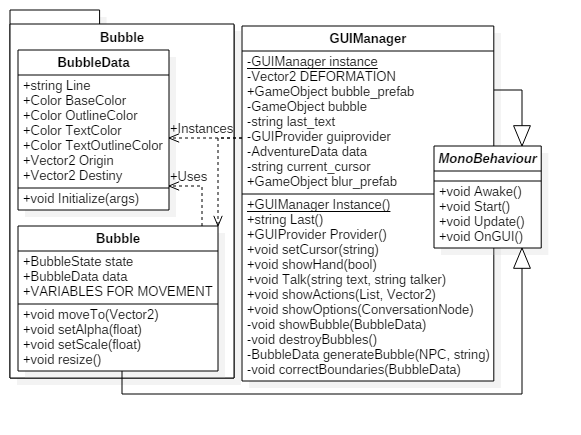
\includegraphics[height=3.5in]{figures/it2/Bubble.png}}
	\caption[Bubble - Versión Final]{Diagrama de clases de Bubble, junto con GUIManager y MonoBehaviour.}
	\label{bubbleit2}
\end{figure}

El proceso de mostrar una burbuja de diálogo comienza en \textit{GUIManager} y es el siguiente: En primer lugar, se identifica si el que habla es el jugador o un personaje, y si es el jugador, se distingue si se trata de un juego en primera persona o un juego en el que el jugador tenga representación en el juego. Una vez se ha determinado quién habla, se obtienen los datos del hablante y se genera una \textit{BubbleData} con dichos datos, decorándola y estableciendo su trayectoria. Este \textit{BubbleData} se pasa a través de una serie de deformaciones que adaptan dichas trayectorias a la pantalla para que no se salga de la misma, y para que se coloque correctamente independientemente de la resolución de la misma. Tras esto se instancia una nueva burbuja en la escena y se delega en ella.

La burbuja, en su función \textit{Start()}, establece su texto en la representación, se prepara para moverse, y se prepara para empezar a mostrarse, pues al principio es transparente. Poco a poco esta se va moviendo y haciéndose visible en su función \textit{FixedUpdate()}, y cuando termina, se queda quieta. Cuando es necesario que la burbuja desaparezca, se ejecuta la función \textit{destroy()} que la hace desaparecer poco a poco, haciéndose más pequeña y transparente.

\subsubsection{Elementos de mejora visual: Apearance}

Existen dos clases que, para mejorar la representación visual del juego, se han desarrollado en el proyecto. Cómo se explicó en el apartado \ref{eandroidmokap} del estado del arte, y visible en la figura \ref{eandroidlupa}, el proyecto eAdventure Android utilizaba mecanismos específicos para ayudar al usuario a encontrar elementos en un entorno táctil. En este proyecto, para ayudar al usuario a encontrar estos elementos, se realiza un brillo de los mismos.

La clase componente \textit{AutoGlower} se encarga de realizar este brillo sobre los objetos que la contengan. Tiene varios modos, como simplemente hacer un flash, o aparecerse y desvanecerse y hacer un flash. Este \textit{AutoGlower} utiliza un \textit{Shader} que genera dicho flash y que es parametrizable para establecer tanto la posición del brillo, su color y su anchura. Este efecto es visible en las figuras \ref{autoglow1it2} y \ref{autoglow2it2};

\begin{figure}[h!]
	\centerline{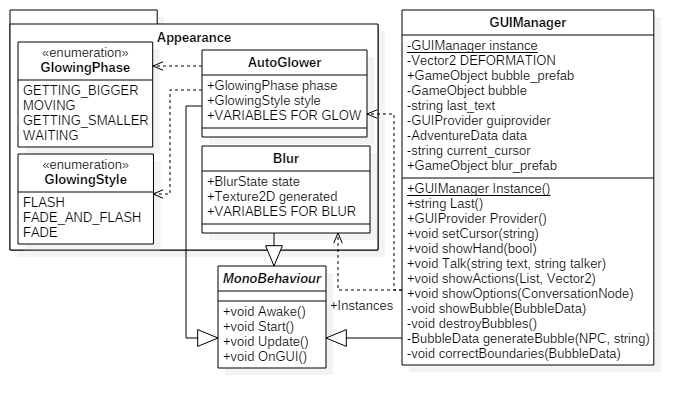
\includegraphics[height=3.5in]{figures/it2/Apearance.png}}
	\caption[Apearance - Versión Final]{Diagrama de clases de Apearance, sin incluir Bubble.}
	\label{apearanceit2}
\end{figure}

Por último, tenemos a la clase \textit{Blur}, que, al igual que la anterior utiliza un \textit{Shader} para conseguir su efecto visual. En este caso, \textit{Blur} lo que hace es volver borroso lo que hay detrás de ella. Es utilizada para generar un cuadrado borroso sobre el cual presentar las distintas opciones disponibles en la lista de opciones de una conversación. Este efecto se puede ver en la figura \ref{blurit2}.

\begin{figure}[h!]
	\centerline{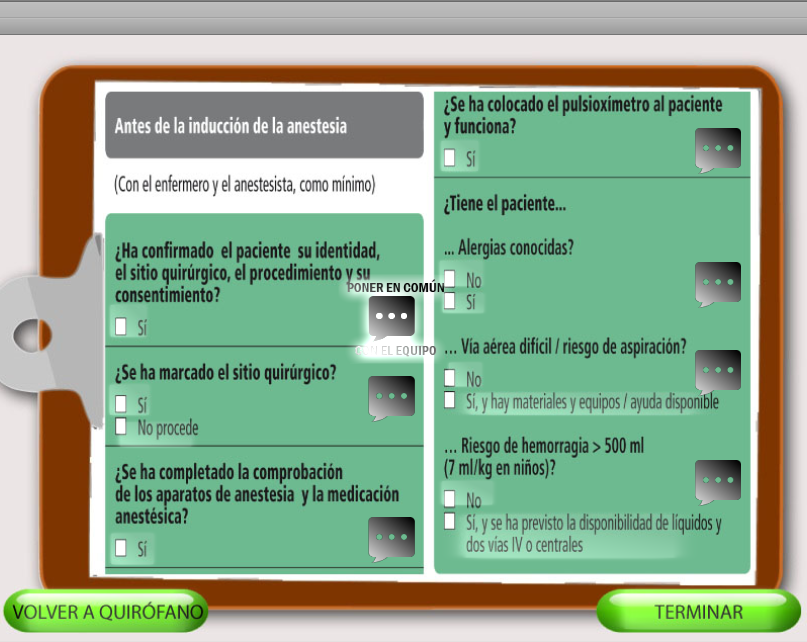
\includegraphics[width=4.3in]{figures/it2/apearance/checklist.png}}
	\caption[Apearance - Versión Final]{Diagrama de clases de Apearance, sin incluir Bubble.}
	\label{autoglow1it2}
\end{figure}

\begin{figure}[h!]
	\centerline{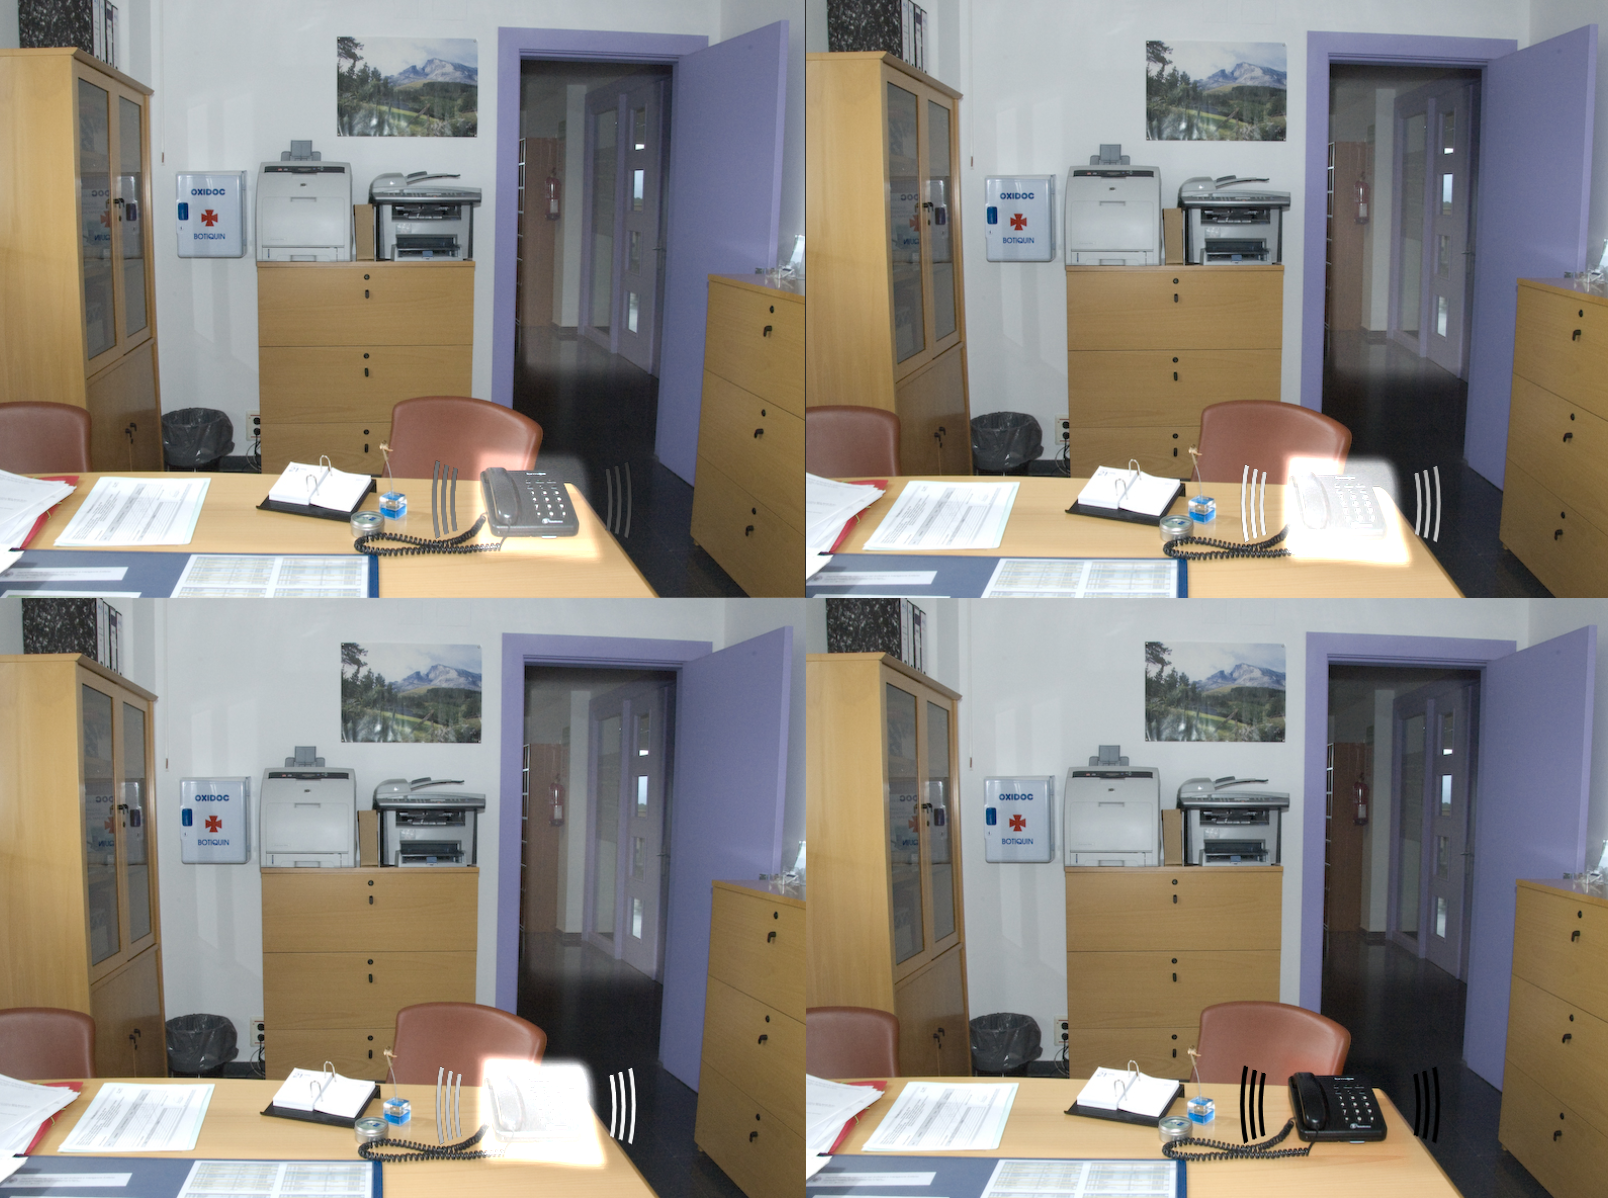
\includegraphics[width=4.3in]{figures/it2/apearance/fire.png}}
	\caption[Apearance - Versión Final]{Diagrama de clases de Apearance, sin incluir Bubble.}
	\label{autoglow2it2}
\end{figure}

\begin{figure}[h!]
	\centerline{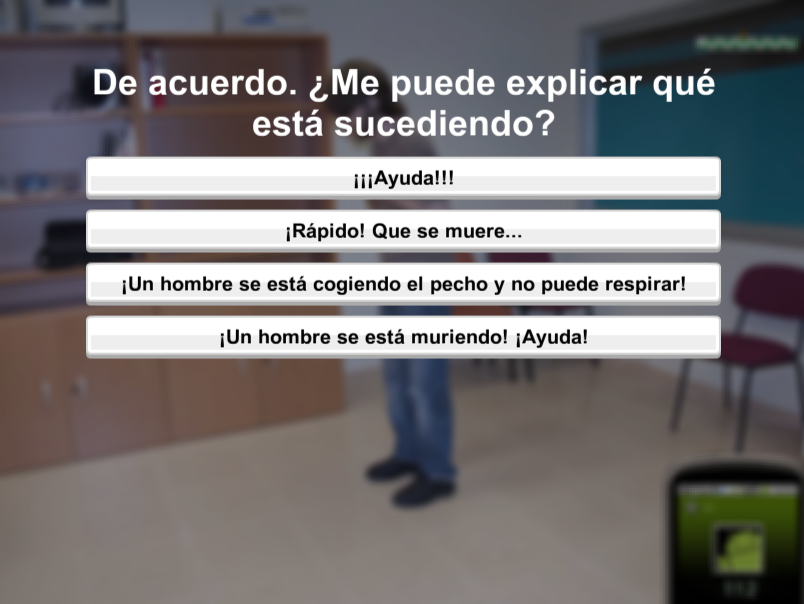
\includegraphics[width=4.3in]{figures/it2/apearance/blur.png}}
	\caption[Apearance - Versión Final]{Diagrama de clases de Apearance, sin incluir Bubble.}
	\label{blurit2}
\end{figure}

\subsubsection{El menú contextual de acciones: Menu}

El menú contextual es uno de los elementos que existían antes y que ha sido recreado, añadiendo animación al mismo para que su representación visual sea más sencilla. La utilidad del menú contextual es mostrar acciones en forma de botones para que el usuario pueda pulsarlos y ejecutar las acciones que están detrás de los mismos.

Este menú contextual se genera utilizando una de las funciones de \textit{GUIManager}, la función \textit{showActions(list<Action>)} que, inicializa el menú y utiliza su función \textit{regenerate()}, que lo que hace es, en función de los parámetros que se le hayan establecido, genera nuevos botones, y los coloca para que se animen correctamente. Tras esto la clase \textit{OptionMB} se encarga de ir colocando tanto la línea que une el centro del menú con el botón, como el botón en si mismo. Asimismo, esta clase establece la acción en \textit{ButtonMB}, clase que implementa la interfaz \textit{Interactuable}, y que permite al usuario interactuar con ella. Es la clase \textit{ButtonMB} la que se encarga de modificar su representación en función de la imagen que le provea el \textit{GUIManager}. Esto está representado en la figura \ref{menuit2}, donde participan \textit{MonoBehaviour} e \textit{Interactuable}.

\begin{figure}[h!]
	\centerline{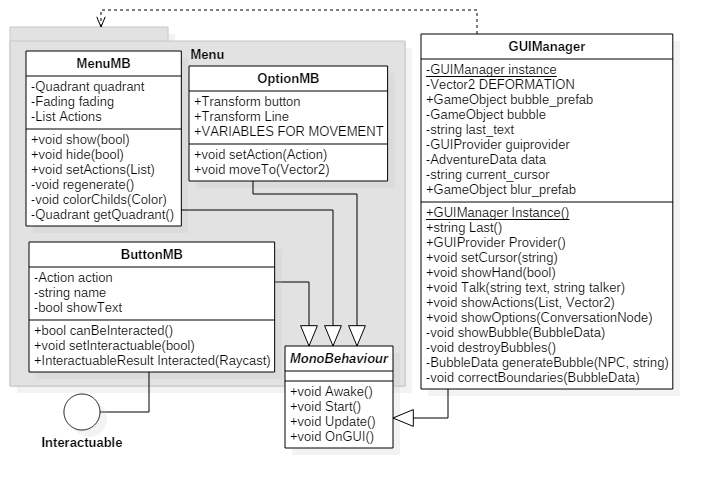
\includegraphics[height=3.3in]{figures/it2/Menu.png}}
	\caption[Menu - Versión Final]{Diagrama de clases de Menu, incluyendo las relaciones que tienen con MonoBehaviour e Interactuable.}
	\label{menuit2}
\end{figure}

Finalmente, en la figura \ref{menuvisualit2} muestra el menú generado en una situación en la que se pueden realizar cinco acciones sobre un elemento de la escena. 

\begin{figure}[h!]
	\centerline{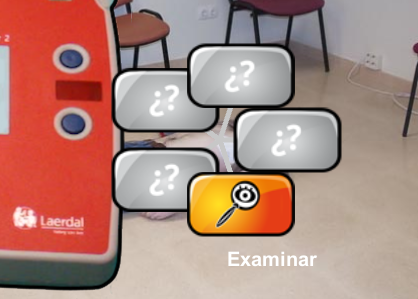
\includegraphics[height=3in]{figures/it2/apearance/menu.png}}
	\caption[Visual Menu - Versión Final]{Imagen de la representación visual del menú.}
	\label{menuvisualit2}
\end{figure}

\subsubsection{El menú contextual de acciones: Menu}

